
\begin{naloga}{Janoš Vidali}{Vaje OR 30.11.2016}
\begin{vprasanje}
Na grafu s slike~\fig izvedi iskanje v širino.
V primerih, ko imaš več ena\-ko\-vred\-nih izbir,
upoštevaj abecedni vrstni red.
Za vsako povezavo določi, ali se nahaja v drevesu iskanja v širino.

\begin{slika}
\pgfslika
\caption{Graf za nalogi~\nal in~\nal[dfs].}
\end{slika}
\end{vprasanje}

\begin{odgovor}
ALGORITEM:\\
\underline{VHOD}:  graf G, vozlišče $s \in V$\\
\underline{IZHOD}: razdalje $d_G(s, v)$ za vsak $v \in V$\\
def bfs(G, s):\\
	\phantom{x}\hspace{3ex}za vsak $v \in V(G)$:\\
		\phantom{x}\hspace{6ex}razdalja[v] = $\infty$\\
	\phantom{x}\hspace{3ex}razdalja[s] = 0\\
	\phantom{x}\hspace{3ex}Q = [s]\\
	\phantom{x}\hspace{3ex}dokler Q ni prazna:\\
		\phantom{x}\hspace{6ex}u = odstrani-prvega(Q)\\
		\phantom{x}\hspace{6ex}za vsak $(u, v) \in E(G)$:\\
			\phantom{x}\hspace{9ex}če razdalja[v] = $\infty$:\\
				\phantom{x}\hspace{12ex}razdalja[v] = razdalja[u] + 1\\
				\phantom{x}\hspace{12ex}vstavi(Q, v)\\
\begin{flushleft}
Če sledimo zgornjemu algoritmu in predpostavki, da upoštevamo vrstni red, začnemo v vozlišču A, je potek sledeč: 
\end{flushleft}
\underline{Predpriprava:}\\
razdalja = $[\infty, \infty, \infty, \infty, \infty, \infty]$\\
razdalja[A] = 0\\
Q = [A]\\
\\
\underline{1. korak:}\\
Odstranimo A iz vrste in pregledamo vse njegove sosede.\\
razdalja[B] = 0 + 1 = 1\\
Q = [B]\\
razdalja[E] = 1\\
Q = [B, E]\\
\\
\underline{2. korak:}\\
Odstranimo B iz vrste in pogledamo vse njegove sosede, ki so še vedno na razdalji $\infty$.\\
razdalja[C] = 1 + 1 = 2\\
Q = [E, C]\\
\\
\underline{3.korak:}\\
Odstranimo E iz vrste.\\
razdalja[F] = 1 + 1 = 2\\
Q = [C, F]\\
\\
\underline{4. korak:}\\
Odstranimo C iz vrste. Ker nima sosedov, ki bi imeli razdaljo še vedno nastavljeno na $\infty$, gremo naprej.\\
Q = [F]\\
\\
\underline{6. korak:}\\
Odstranimo F iz vrste.\\
razdalja[I] = 3\\
Q = [I]\\
\\
\underline{6. korak:}\\
Odstranimo I iz vrste. Ker nima sosedov na razdalji $\infty$, gremo naprej.\\
\\
\underline{7. korak:}\\
Ker je na tej točki vrsta prazna, se algoritem ustavi.\\
\\
\begin{flushleft}
Podobno naredimo za drugi del grafa. Ker nista povezana, moramo algoritem začeti od začetka. 
\end{flushleft}
\underline{Predpriprava:}\\
razdalja = $[\infty, \infty, \infty]$\\
razdalja[D] = 0\\
Q = [D]\\
\\
\underline{1. korak:}\\
Iz vrste odstranimo D.\\
razdalja[G] = 1\\
Q = [G]\\
razdalja[H] = 1\\
Q = [G, H]\\
\\
\underline{2. korak:}\\
Odstranimo G iz vrste. Ker nima sosedov na razdalji $\infty$, gremo naprej.\\
\\
\underline{3. korak:}\\
Odstranimo H iz vrste. Ker nima sosedov na razdalji $\infty$, gremo naprej.\\
\\
\underline{4. korak:}\\
Ker je na tej točki vrsta prazna, se algoritem ustavi.
\newpage
\begin{flushleft}
Drevo iskanja v širino: 
\end{flushleft}
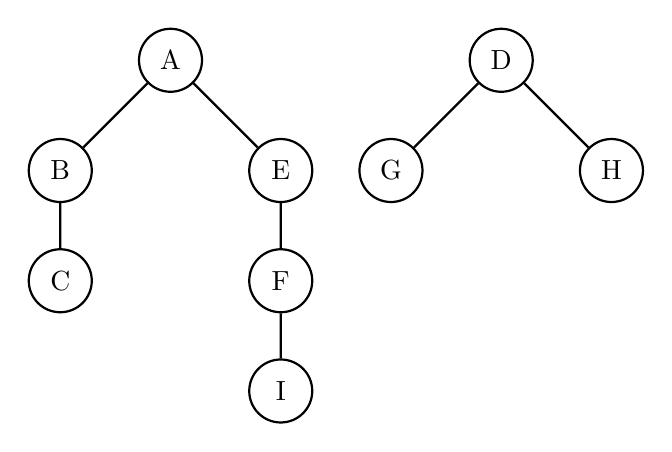
\begin{tikzpicture}[style=thick,scale=0.7]
\tikzstyle{vertex}=[draw, circle, fill=white, inner sep=0pt, minimum size=8mm]

\node[vertex] (A) at (-2, 2) {A};
\node[vertex] (B) at ( -4, 0) {B};
\node[vertex] (C) at ( -4, -2) {C};
\node[vertex] (D) at ( 4, 2) {D};
\node[vertex] (E) at ( 0, 0) {E};
\node[vertex] (F) at ( 0, -2) {F};
\node[vertex] (G) at ( 2, 0) {G};
\node[vertex] (H) at ( 6, 0) {H};
\node[vertex] (I) at ( 0, -4) {I};

\draw (A) -- (B) -- (C);
\draw (A) -- (E) -- (F) -- (I);
\draw (D) -- (G);
\draw (D) -- (H);
\end{tikzpicture}
\\
\\
\begin{flushleft}
Torej iz zgornjega drevesa jasno vidimo, da so drevesne povezave: (A, B), (B, C), (A, E), (E, F), (F, I), (D, G), (D, H).
\end{flushleft}

\end{odgovor}
\end{naloga}
